\documentclass[aspectratio=169,11pt]{beamer}
\usepackage[T1]{fontenc}
\usepackage[utf8]{inputenc}
\usepackage{lmodern,amsmath,amssymb,booktabs,tikz}
\usetikzlibrary{positioning,arrows.meta}
\usepackage[authoryear,round]{natbib}
\bibpunct{(}{)}{;}{a}{}{,}
\graphicspath{{figures/backtest/}}

\definecolor{Ink}{HTML}{15263C}
\definecolor{Teal}{HTML}{007A75}
\definecolor{Paper}{HTML}{F3F7FA}
\setbeamercolor{normal text}{fg=Ink,bg=white}
\setbeamercolor{structure}{fg=Teal}
\setbeamercolor{frametitle}{fg=white,bg=Ink}
\setbeamercolor{block title}{fg=white,bg=Teal}
\setbeamercolor{block body}{fg=Ink,bg=Paper}
\setbeamertemplate{navigation symbols}{}
\setbeamertemplate{bibliography item}{}
\setbeamercolor{bibliography entry author}{fg=Ink}
\setbeamercolor{bibliography entry title}{fg=Ink}
\setbeamercolor{bibliography entry location}{fg=Teal}
\setbeamercolor{bibliography entry note}{fg=Teal}
\setbeamertemplate{footline}{%
  \hfill\color{Teal}\insertframenumber\,/\,\inserttotalframenumber
  \hspace{5mm}\vspace{2mm}}
\setbeamersize{text margin left=8mm,text margin right=8mm}

\newcommand{\repo}{https://github.com/michalmarchwiak/bsc-project}
\newcommand{\rev}{9e941db56fde866672b262f5f6725268ce58feb7}
\newcommand{\src}[2]{\vfill{\scriptsize\color{Teal}%
  \href{\repo/blob/\rev/#1}{#2}}}
\newcommand{\srcmain}[2]{\vfill{\scriptsize\color{Teal}%
  \href{\repo/blob/main/#1}{#2}}}
\newcommand{\zespol}{Łukasz Banik, Jakub Bartłomowicz, Michał Marchwiak, Michał Pluciński}
\newcommand{\ind}{\mathbf{1}}
\newcommand{\E}{\mathbb{E}}

\begin{document}

% ============================================================ wstęp
\begin{frame}[plain]
  {\color{Teal}\textbf{POLITECHNIKA WROCŁAWSKA}}\par
  Matematyka stosowana \hfill Projekt inżynierski
  \vfill
  {\LARGE\bfseries
    Analiza ryzyka funduszu inwestycyjnego\par
    z uwzględnieniem zależności aktywów\par}
  \vspace{4mm}
  {\color{Teal}\rule{27mm}{1.2pt}}
  \vfill
  \zespol\par
\end{frame}

\begin{frame}{Jak wspólne spadki zmieniają ryzyko funduszu?}
  \begin{block}{Pytanie badawcze}
    Jak wybór modelu zależności wpływa na prognozowane straty
    funduszu oraz na jego wyniki po rebalansowaniu?
  \end{block}
  \begin{itemize}
    \item \textbf{Model danych.} Rozkład łączny stóp zwrotu
      \(F(r_1,\dots,r_d)=C\bigl(F_1(r_1),\dots,F_d(r_d)\bigr)\):
      osobno marginesy \(F_i\), osobno kopuła \(C\) (tw.\ Sklara;
      \citealp{sklar1959}). Korelacja liniowa nie opisuje
      zależności w ogonach \citep{embrechts2002}.
    \item \textbf{Decyzja.} Wagi maksymalizują ekwiwalent pewności
      funkcji użyteczności CRRA z karą za zależność w dolnym ogonie.
    \item \textbf{Ocena ryzyka.} VaR i ES z symulacji Monte Carlo,
      weryfikowane na zrealizowanych stratach i bootstrapem ex post.
  \end{itemize}
  \src{README.md}{Cel projektu i zestaw modeli}
\end{frame}

\begin{frame}{Dane i struktura funduszu}
  \begin{columns}[T,onlytextwidth]
    \column{.50\textwidth}
    \textbf{Dane wejściowe}
    \begin{itemize}
      \item Notowania dzienne 2005--2026 (Yahoo, Stooq), kursy NBP,
        warunki emisji obligacji oszczędnościowych.
      \item Dzienne log-stopy w PLN:
        \(r_{i,t}=\ln P_{i,t}-\ln P_{i,t-1}\).
      \item WIBOR 1M jako stopa wolna od ryzyka.
      \item Aktywa USA przeliczone na PLN zawierają ryzyko
        walutowe \citep{kurach2016}.
    \end{itemize}
    \column{.47\textwidth}
    \textbf{Struktura dwupoziomowa}
    \[
      x=\sum_{k=1}^{10}W_k\,w_k ,
    \]
    \(w_k\) -- wagi instrumentów w subfunduszu \(k\),
    \(W_k\) -- waga subfunduszu,
    \(x\) -- ekspozycja \emph{look-through} na instrumenty.
    \begin{itemize}
      \item SF1--SF9: ok.\ 80 instrumentów w dacie,
        SF10: 8 rodzin obligacji oszczędnościowych.
    \end{itemize}
  \end{columns}
  \src{config/subfunds.yaml}{Konfiguracja subfunduszy i reguły doboru aktywów}
\end{frame}

% ============================================================ modelowanie danych
\begin{frame}{Modelowanie danych (1): rozkłady brzegowe}
  Dla każdego instrumentu, w oknie 1260 sesji przed datą decyzji:
  \[
    \begin{aligned}
      r_t &= \mu+\phi\,r_{t-1}+\varepsilon_t,
        \qquad \varepsilon_t=\sigma_t z_t,
        \qquad z_t\sim \text{skew-}t(\eta,\lambda),\\
      \sigma_t^2 &= \omega+\bigl(\alpha+\delta\,\ind\{\varepsilon_{t-1}<0\}\bigr)
        \varepsilon_{t-1}^2+\beta\,\sigma_{t-1}^2 .
    \end{aligned}
  \]
  \begin{itemize}
    \item AR(1) opisuje średnią, GJR-GARCH(1,1) -- skupianie zmienności
      i asymetrię (\(\delta>0\): spadki zwiększają zmienność bardziej
      niż wzrosty; \citealp{glosten1993}; dla rynków CEE:
      \citealp{botoc2017}).
    \item Skośny rozkład \(t\) \citet{hansen1994}: grube ogony (\(\eta\)) i
      skośność (\(\lambda\)).
    \item Estymacja MNW (pakiet \texttt{arch}, \citealp{arch});
      standaryzowane reszty
      \(\hat z_t=\hat\varepsilon_t/\hat\sigma_t\) są w przybliżeniu iid
      i przenoszą informację o zależności \citep{mcneil2000}.
    \item SF10: margines deterministyczny, \(r_h=\hat\mu\) (średnia z 21
      sesji), poza kopułą.
  \end{itemize}
  \src{src/pf/models/margins.py}{Marginesy AR(1)--GJR-GARCH skew-t}
\end{frame}

\begin{frame}{Modelowanie danych (2): pseudoobserwacje i agregacja}
  \begin{columns}[T,onlytextwidth]
    \column{.52\textwidth}
    \textbf{Agregacja 5-dniowa}
    \[
      s_{i,t}=\sum_{j=0}^{k-1}\hat z_{i,t-j},\qquad k=5,
    \]
    \[
      \operatorname{cov}(s_i,s_j)=k\,\gamma_{ij}(0)
        +(k-1)\bigl(\gamma_{ij}(1)+\gamma_{ji}(1)\bigr).
    \]
    GPW (17:00), NYSE (22:00) i fixing NBP (11:50) nie są
    synchroniczne. Suma obejmuje zależność opóźnioną o sesję.
    \column{.45\textwidth}
    \textbf{Pseudoobserwacje}
    \[
      \hat u_{i,t}=\frac{\operatorname{rank}(s_{i,t})}{n+1}\in(0,1).
    \]
    \begin{itemize}
      \item Podejście półparametryczne: kopuła nie zależy od
        błędnej specyfikacji marginesu.
      \item Wspólne pseudoobserwacje dla wszystkich 7 modeli
        zależności \(\Rightarrow\) porównanie bez wpływu marginesów.
    \end{itemize}
  \end{columns}
  \src{docs/dependence_model.md}{Panel reszt i agregacja}
\end{frame}

\begin{frame}{Modelowanie danych (3): kopuły winoroślowe}
  Gęstość R-vine to iloczyn kopuł parowych po krawędziach drzew
  \(T_1,\dots,T_L\):
  \[
    c(u_1,\dots,u_d)=\prod_{\ell=1}^{L}\ \prod_{e\in T_\ell}
      c_{a_e b_e\mid D_e}\Bigl(F(u_{a_e}\mid u_{D_e}),\,
                              F(u_{b_e}\mid u_{D_e})\Bigr),
  \]
  a warunkowe dystrybuanty liczymy rekurencyjnie \(h\)-funkcjami
  \(h(u\mid v)=\partial C(u,v)/\partial v\)
  \citep{bedford2002,aas2009}.
  \begin{itemize}
    \item Struktura: algorytm \citet{dissmann2013} (maks.\ drzewa rozpinające
      z wagami \(|\hat\tau_{\text{Kendall}}|\)), obcięcie na \(L=3\).
    \item Rodziny: Gauss, \(t\), Clayton, Gumbel (z obrotami), Frank;
      wybór AIC, sekwencyjna MNW.
    \item Porównanie: R-, C-, D-vine, Gauss, \(t\)-Student,
      niezależność, empiryczna; AIC/BIC, test \citet{vuong1989},
      log-score poza próbą; por.\ \citet{muller2024}.
  \end{itemize}
  \src{src/pf/models/rvine.py}{Estymacja R-vine}
\end{frame}

\begin{frame}{Od kopuły do scenariuszy Monte Carlo}
  \centering
  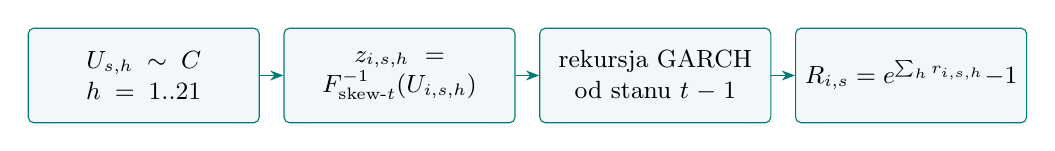
\begin{tikzpicture}[
    node distance=3mm,
    box/.style={draw=Teal,fill=Paper,rounded corners=2pt,
      text width=27mm,align=center,minimum height=12mm,font=\small},
    >=Stealth]
    \node[box] (a) {\(U_{s,h}\sim C\)\\ \(h=1..21\)};
    \node[box,right=of a] (b) {\(z_{i,s,h}=F^{-1}_{\text{skew-}t}(U_{i,s,h})\)};
    \node[box,right=of b] (c) {rekursja GARCH od stanu \(t-1\)};
    \node[box,right=of c] (d) {\(R_{i,s}=e^{\sum_h r_{i,s,h}}-1\)};
    \draw[->,Teal] (a)--(b);
    \draw[->,Teal] (b)--(c);
    \draw[->,Teal] (c)--(d);
  \end{tikzpicture}
  \raggedright\medskip
  \begin{itemize}
    \item Wynik: macierz scenariuszy \(R\in\mathbb{R}^{N\times d}\)
      miesięcznych prostych stóp zwrotu (PLN).
    \item Wspólne liczby losowe \(U\) dla wszystkich modeli
      \(\Rightarrow\) różnice wynikają z kopuły, nie z szumu MC.
    \item Adaptacyjne \(N\) (partie po 2500, \(N\le 50\,000\)), stop gdy
      \(\mathrm{SE}(\widehat{\mathrm{ES}})/|\widehat{\mathrm{ES}}|\le 2\%\):
      \[
        \mathrm{SE}(\widehat{\mathrm{ES}}_\alpha)=
        \sqrt{\frac{\operatorname{Var}(L\mid L>\mathrm{VaR}_\alpha)
          +\alpha(\mathrm{ES}_\alpha-\mathrm{VaR}_\alpha)^2}{(1-\alpha)N}}.
      \]
  \end{itemize}
  \src{src/pf/sim/scenarios.py}{Symulacja scenariuszy i estymacja ES}
\end{frame}

\begin{frame}{Miary ryzyka: VaR i ES}
  Strata portfela w scenariuszu \(s\):
  \[
    L_s=-\sum_{i=1}^d x_i R_{s,i},
    \qquad
    \mathrm{VaR}_\alpha(L)=q_\alpha(L),
    \qquad
    \mathrm{ES}_\alpha(L)=\frac{1}{1-\alpha}\int_\alpha^1 q_u(L)\,du .
  \]
  \begin{columns}[T,onlytextwidth]
    \column{.47\textwidth}
    \textbf{VaR} -- próg straty przekraczany z prawd.\ \(1-\alpha\).
    Nie jest subaddytywny.
    \column{.50\textwidth}
    \textbf{ES} -- średnia strata w najgorszych \(1-\alpha\)
    scenariuszach. Miara koherentna \citep{artzner1999,acerbi2002},
    wypukła w wagach.
  \end{columns}
  \medskip
  Empirycznie:
  \(\widehat{\mathrm{ES}}_\alpha=\frac{1}{\lceil(1-\alpha)N\rceil}
  \sum_{s\in\text{ogon}}L_s\).
  Poziom w backteście: \(\alpha=97{,}5\%\), horyzont 21 sesji
  \citep[rozdz.~2]{mcneil2005}.
  \src{src/pf/opt/cvar.py}{Empiryczne VaR i ES}
\end{frame}

% ============================================================ użyteczność i optymalizacja
\begin{frame}{Funkcja użyteczności CRRA i ekwiwalent pewności}
  \begin{columns}[T,onlytextwidth]
    \column{.55\textwidth}
    Użyteczność majątku \(g=1+R^\top w\):
    \[
      u_\gamma(g)=\frac{g^{1-\gamma}}{1-\gamma},\qquad
      u_1(g)=\ln g,
    \]
    względna awersja do ryzyka \(-g\,u''/u'=\gamma\) jest stała
    \citep{pratt1964}.
    Ekwiwalent pewności na scenariuszach:
    \[
      \mathrm{CE}_\gamma(w)=\Bigl(\tfrac1N\sum_{s}
        (1+R_s^\top w)^{1-\gamma}\Bigr)^{\frac{1}{1-\gamma}}-1 .
    \]
    \column{.42\textwidth}
    \begin{itemize}
      \item \(u_\gamma(1+\mathrm{CE})=\E\,u_\gamma(1+R^\top w)\):
        pewna stopa równoważna loterii.
      \item \(\mathrm{CE}_\gamma\) to średnia potęgowa rzędu
        \(1-\gamma<1\) \(\Rightarrow\) wklęsła w \(w\),
        \(\mathrm{CE}_\gamma\le\E[R^\top w]\).
      \item Gradient analityczny, liczenie w logarytmach
        (log-sum-exp) dla dużych \(\gamma\).
      \item Uwzględnia wszystkie momenty, w tym ogony,
        a nie tylko \(\mu\) i \(\sigma^2\).
    \end{itemize}
  \end{columns}
  \src{src/pf/opt/utility.py}{CE i gradient}
\end{frame}

\begin{frame}{Kara za zależność w dolnym ogonie}
  Pseudoobserwacje scenariuszy \(V_{s,i}=\operatorname{rank}(R_{s,i})/(N+1)\):
  \[
    \Lambda_{ij}(q)=\frac{1}{Nq}\sum_{s=1}^N
      \ind\{V_{s,i}\le q\}\,\ind\{V_{s,j}\le q\},\qquad q=0{,}05,
  \]
  czyli oszacowanie \(P(V_j\le q\mid V_i\le q)\): prawdopodobieństwa
  wspólnego spadku. \(\Lambda=I^\top I/(Nq)\) jest PSD.
  \[
    \max_w\ \mathrm{CE}_\gamma(w)-\kappa\,\sigma^{EW}\,w^\top\Lambda(q)\,w
  \]
  \begin{itemize}
    \item Funkcja celu jest wklęsła \(\Rightarrow\) optimum globalne
      (SLSQP z gradientem \(\nabla D=2\Lambda w\);
      \citealp{scipy2020}).
    \item Niezależne aktywa: \(\Lambda_{ij}\approx q\); komonotoniczne:
      \(\Lambda_{ij}=1\). SF10 (stała stopa) ma \(\Lambda_{ij}=0\).
    \item \(\sigma^{EW}\) skaluje karę do zmienności portfela równych wag.
  \end{itemize}
  \src{src/pf/opt/dependence_penalty.py}{Macierz zależności w ogonie}
\end{frame}

\begin{frame}{Profile inwestora}
  \centering
  \begin{tabular}{llrrrrrr}
    \toprule
    Profil & & \(\gamma\) & \(\kappa\) & \(c_{SF}\) & \(c_{LT}\)
      & \(c_{LT}/c_{SF}\) & \(W_{\max}\)\\
    \midrule
    P1 & konserwatywny & 10  & 1,00 & 0,20 & 0,05 & 0,25  & 0,20\\
    P2 & umiarkowany   & 7   & 0,60 & 0,25 & 0,07 & 0,28  & 0,225\\
    P3 & zrównoważony  & 5   & 0,35 & 0,30 & 0,10 & 0,33  & 0,25\\
    P4 & dynamiczny    & 3   & 0,15 & 0,40 & 0,15 & 0,375 & 0,60\\
    P5 & agresywny     & 1,5 & 0,05 & 0,50 & 0,25 & 0,50  & 0,75\\
    \bottomrule
  \end{tabular}
  \raggedright\medskip
  \begin{itemize}
    \item \(\gamma\) -- awersja do ryzyka, \(\kappa\) -- waga kary za
      zależność w ogonie.
    \item \(c_{SF}\) -- limit wagi instrumentu w subfunduszu,
      \(c_{LT}\) -- limit ekspozycji look-through,
      \(W_{\max}\) -- limit wagi subfunduszu.
    \item \(W_k\le\min(W_{\max},c_{LT}/m_k)\), więc \(W_{\max}\) wiąże
      tylko poniżej \(c_{LT}/c_{SF}\): dla P1--P3 ustawiono go poniżej
      tego progu.
    \item Wyniki na kolejnych slajdach: przebieg \texttt{7d0ff370e76f}
      z powyższymi limitami.
  \end{itemize}
  \src{config/profiles.yaml}{Parametry profili}
\end{frame}

\begin{frame}{Optymalizacja dwupoziomowa i ograniczenie look-through}
  \textbf{Poziom 1} (każdy subfundusz \(k\), scenariusze jego aktywów \(R^{(k)}\)):
  \[
    w_k^*=\arg\max_{w}\ \mathrm{CE}_\gamma(w)-\kappa\sigma_k^{EW}w^\top\Lambda_k w,
    \quad \mathbf 1^\top w=1,\quad 0\le w_i\le\max(c_{SF},1/n_k).
  \]
  \textbf{Poziom 2} (scenariusze subfunduszy \(R^{SF}_{s,k}=R^{(k)}_s w_k^*\)):
  \[
    W^*=\arg\max_{W}\ \mathrm{CE}_\gamma(W)-\kappa\sigma^{EW}_{SF}W^\top\Lambda^{SF}W,
    \quad \mathbf 1^\top W=1,\quad 0\le W_k\le u_k .
  \]
  \textbf{Look-through:}
  \(x_i=W_k w_{k,i}\le c_{LT}\ \Leftrightarrow\
    W_k\le u_k=\min\bigl(W_{\max},\,c_{LT}/m_k\bigr),\ m_k=\max_i w_{k,i}^*\).
  \begin{itemize}
    \item Limit nieliniowy staje się zwykłym ograniczeniem pudełkowym.
    \item Gdy \(\sum_k u_k<1\): \(c_{LT}\to s\,c_{LT}\) z minimalnym
      \(s\ge1\) (luzowanie proporcjonalne).
    \item Dekompozycja jest heurystyką, a nie optimum łącznym względem \(x\).
  \end{itemize}
  \src{src/pf/opt/profiles.py}{Optymalizacja dwupoziomowa i look-through}
\end{frame}

\begin{frame}{Strategie porównawcze: minimalizacja ES jako LP}
  Dla \(N\) jednakowo prawdopodobnych scenariuszy \citep{rockafellar2000}:
  \[
    \begin{aligned}
      \min_{w,\,z,\,u}\quad &
        z+\frac{1}{N(1-\alpha)}\sum_{s=1}^{N}u_s\\
      \text{przy}\quad &
        u_s\ge -R_s^\top w-z,\qquad u_s\ge 0,\quad s=1,\dots,N,\\
      & \mathbf{1}^\top w=1,\qquad 0\le w_i\le \overline w_i.
    \end{aligned}
  \]
  \begin{itemize}
    \item \texttt{min\_es}: powyższy LP; \texttt{maxret\_es}:
      \(\max \E[R^\top w]\) przy \(\mathrm{ES}_\alpha(w)\le\mathrm{ES}_\alpha(w^{EW})\).
    \item \texttt{ce}: \(\kappa=0\); \texttt{ce\_dep}: z karą
      za zależność (strategia główna).
    \item Benchmarki: równe wagi, średnia--wariancja
      (\(\max\mu^\top w-\tfrac\gamma2 w^\top\Sigma w\), \(\Sigma\) wg \citealp{ledoit2004}),
      SPY, WIG20TR.
  \end{itemize}
  \src{src/pf/opt/cvar.py}{Implementacja optymalizacji opartej na ES}
\end{frame}

% ============================================================ reewaluacja
\begin{frame}{Reewaluacja subfunduszy co miesiąc}
  W pierwszej sesji każdego miesiąca, na danych do \(t-1\):
  \begin{enumerate}
    \item \textbf{Skład uniwersum.} Raz w roku (styczeń) wybór spółek
      SF1, SF2, SF8, SF9 wg obrotu z 12 miesięcy; tylko dane sprzed \(t\).
    \item \textbf{Ponowna estymacja} marginesów i kopuł w oknie 1260 sesji
      i nowe scenariusze.
    \item \textbf{Nowe wagi} \(w_k^*\) i \(W^*\) -- obie warstwy liczone od nowa.
    \item \textbf{Transakcja} na zamknięciu \(t\), dalej kupno i trzymanie.
  \end{enumerate}
  Dryf wag i koszt przejścia z \(\tilde x\) do \(x_t\):
  \[
    \tilde x_{i}=\frac{x_{t-1,i}\prod_j(1+r_{i,j})}{V},\qquad
    k_t=c\sum_i|x_{t,i}-\tilde x_i|+\sum_i f_i(t)\,(\tilde x_i-x_{t,i})^+,
  \]
  \(c=0{,}1\%\), \(f_i\) -- opłata za wcześniejszy wykup obligacji SF10;
  \(r^{\text{net}}_t=(1-k_t)(1+r^{\text{brutto}}_t)-1\).
  \src{src/pf/backtest/realized.py}{Realizacja stóp, dryf i koszty}
\end{frame}

\begin{frame}{Skład subfunduszy w czasie (poziom 1)}
  \centering
  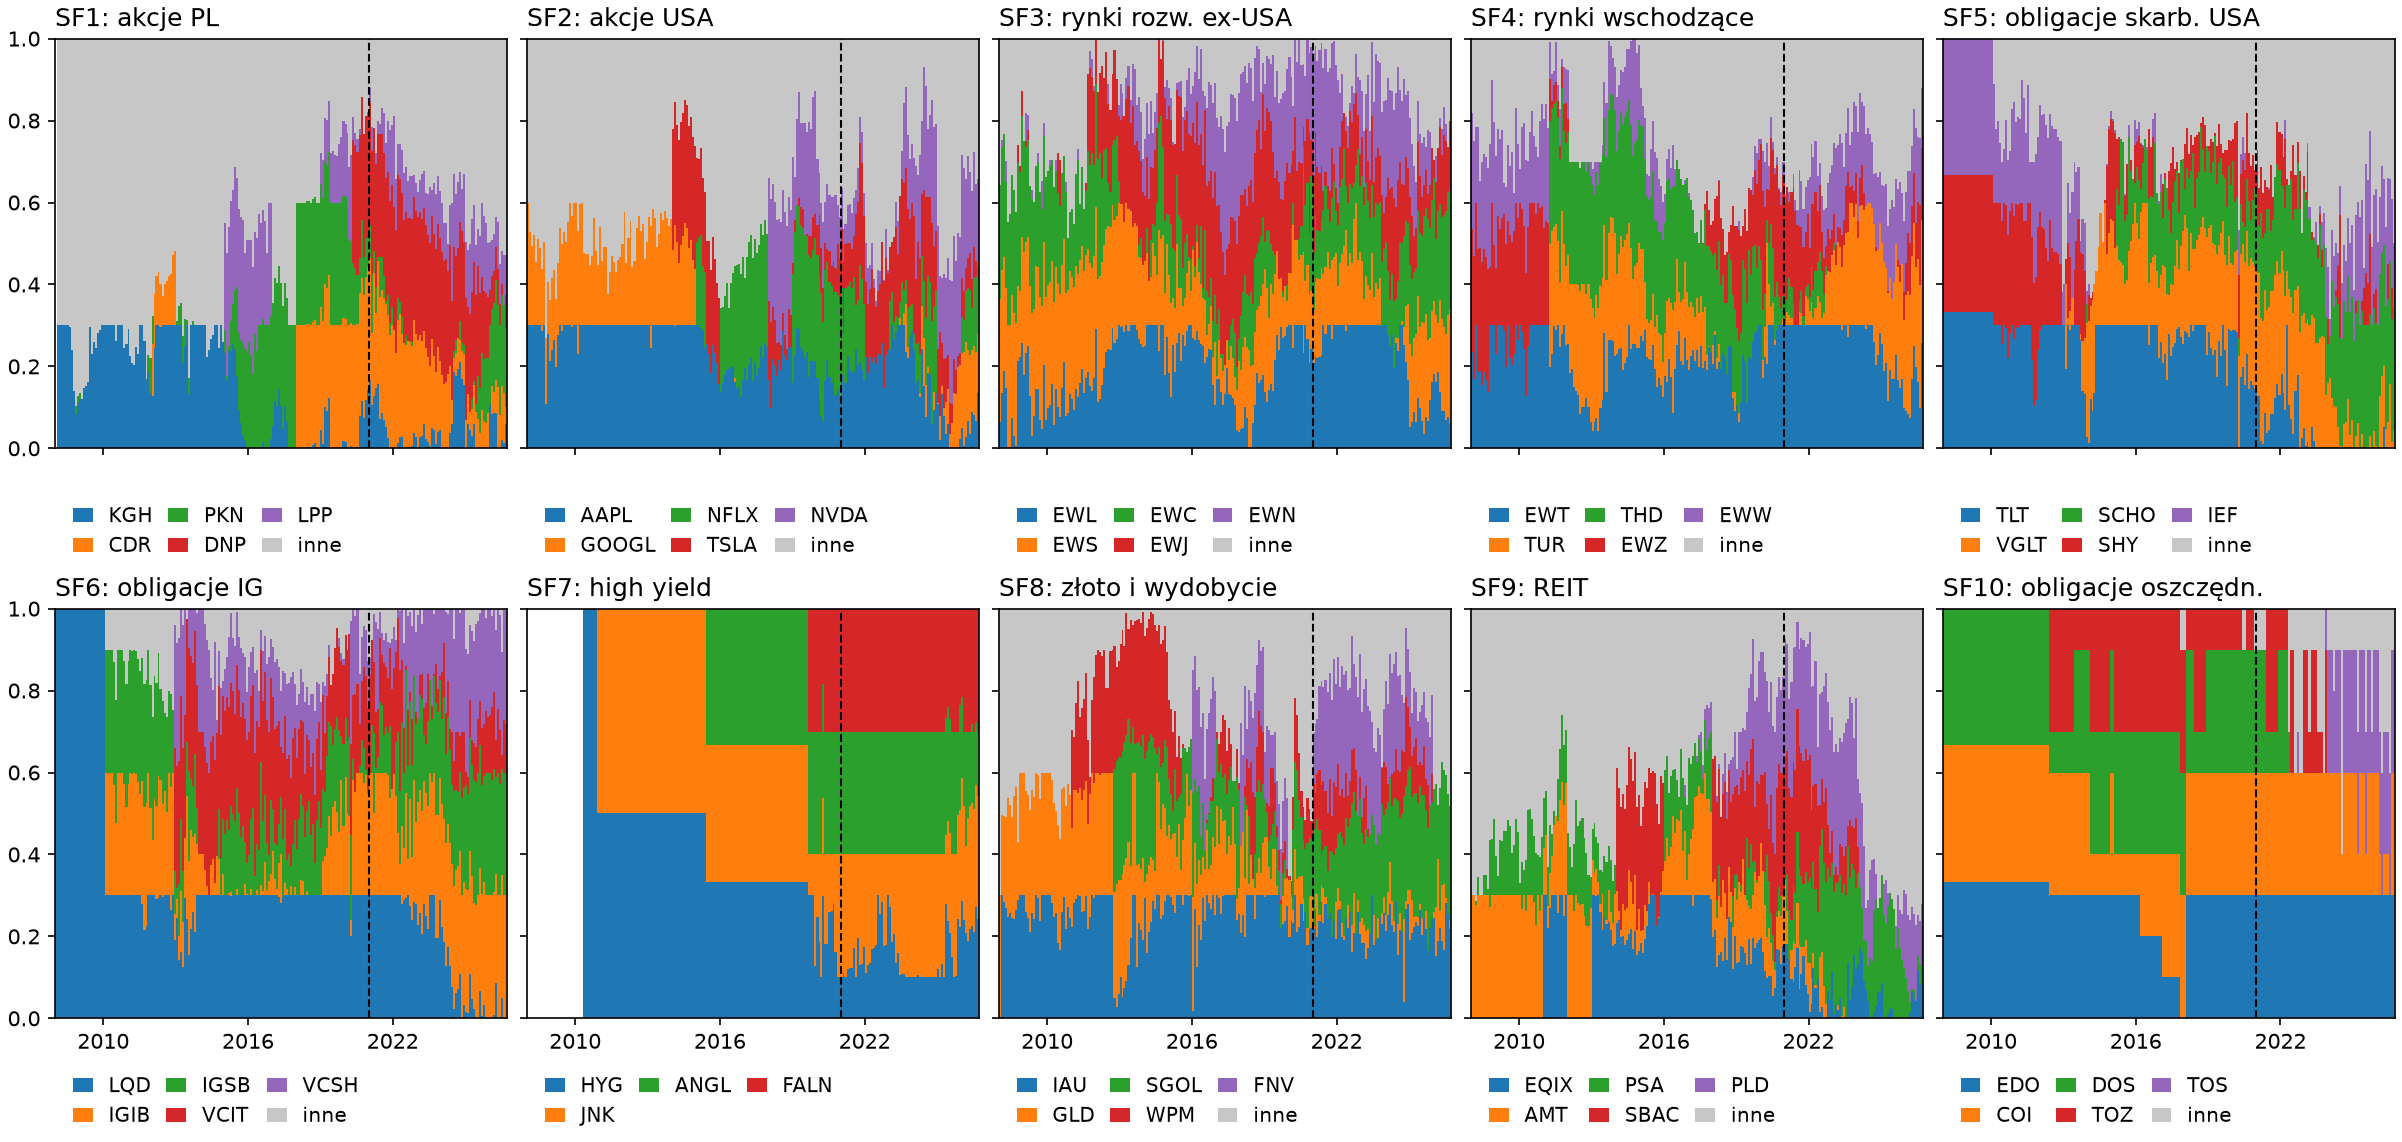
\includegraphics[width=.93\textwidth]{subfund_composition_P3.png}\par
  {\scriptsize R-vine \(\times\) \texttt{ce\_dep}, profil P3; 5 instrumentów
    o największej średniej wadze, reszta jako „inne”.}
  \srcmain{pipelines/composition_figures.py}{Kod wykresu: pipelines/composition\_figures.py}
\end{frame}

\begin{frame}{Struktura portfela w czasie (poziom 2): P1--P3}
  \centering
  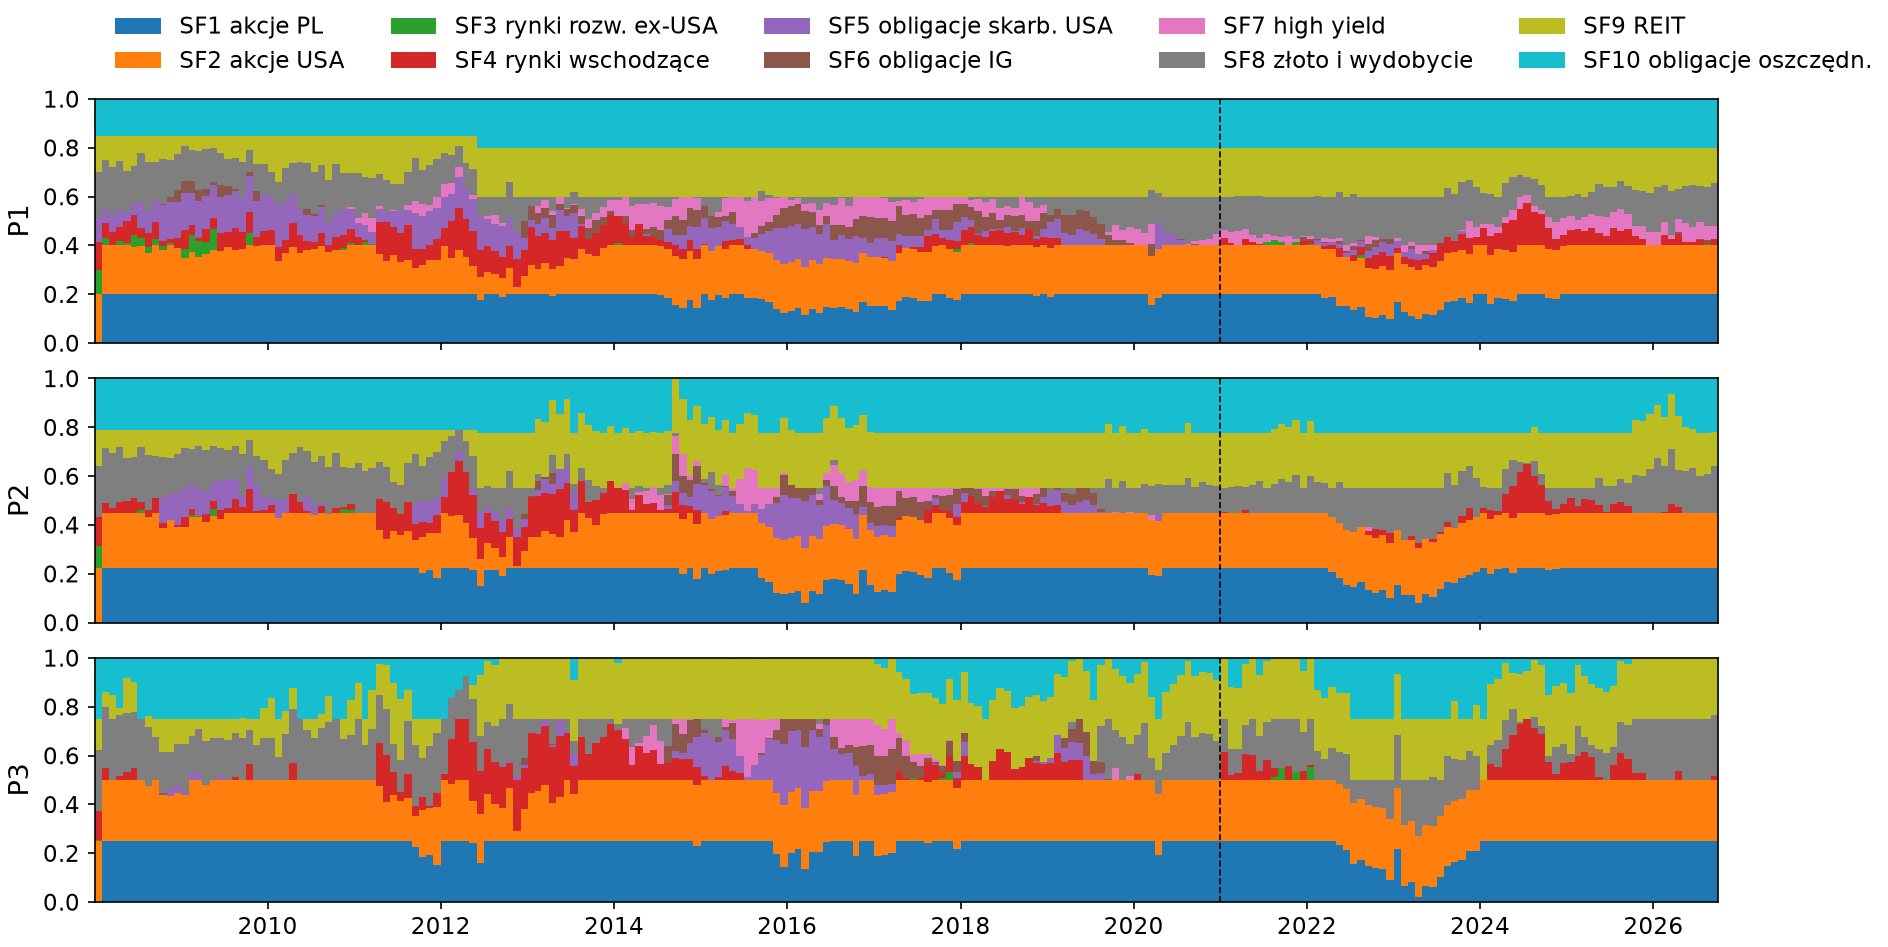
\includegraphics[width=\textwidth,height=.72\textheight,keepaspectratio]{portfolio_W_P1-P3.png}\par
  {\scriptsize Wagi subfunduszy \(W_k\), R-vine \(\times\) \texttt{ce\_dep};
    linia przerywana: początek hold-outu.}
  \srcmain{pipelines/composition_figures.py}{Kod wykresu: pipelines/composition\_figures.py}
\end{frame}

\begin{frame}{Struktura portfela w czasie (poziom 2): P4--P5}
  \centering
  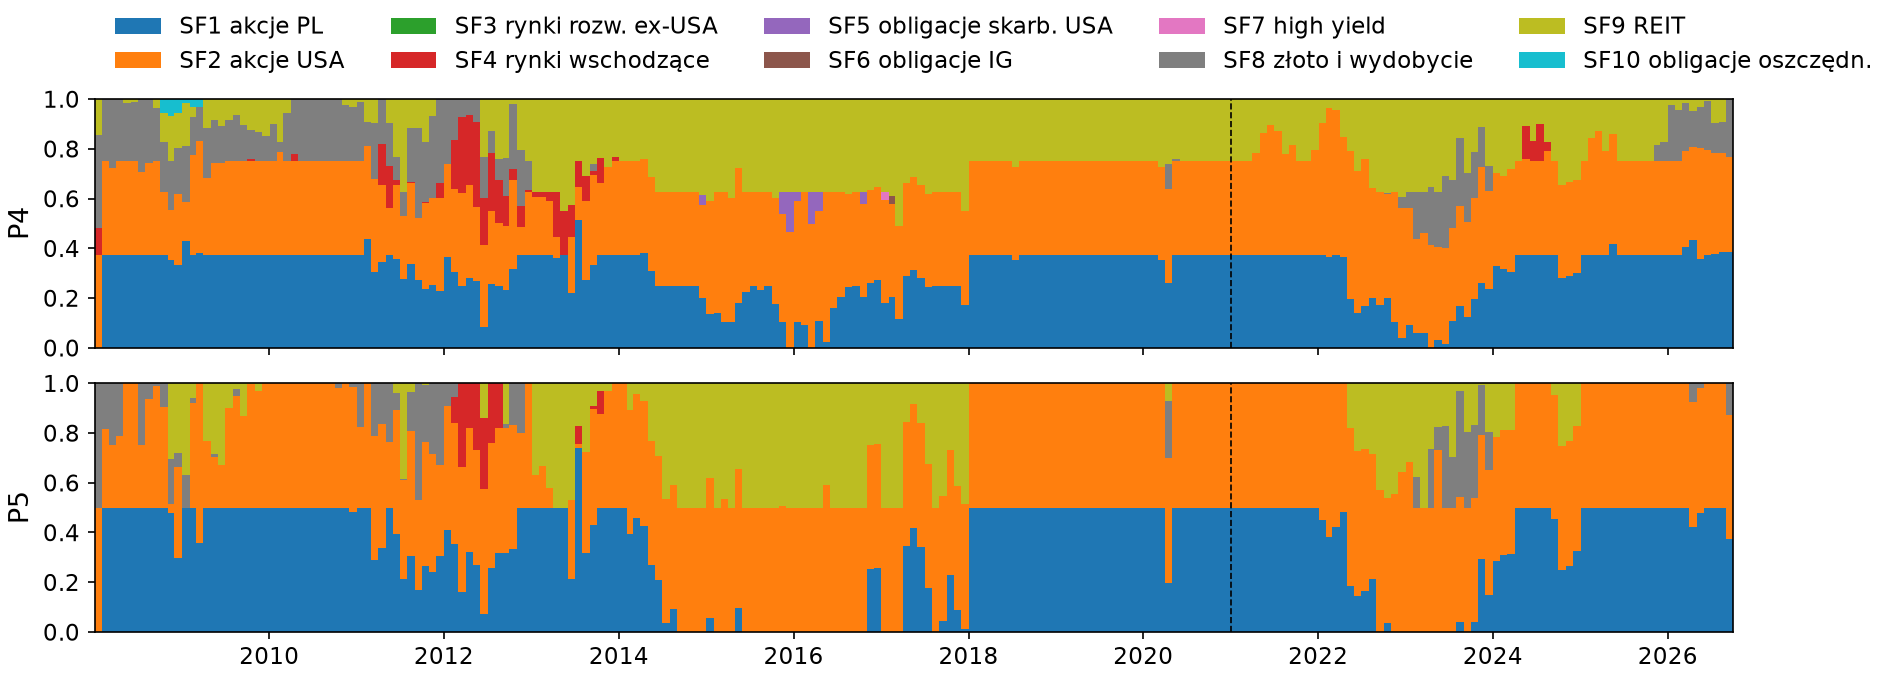
\includegraphics[width=\textwidth,height=.72\textheight,keepaspectratio]{portfolio_W_P4-P5.png}\par
  {\scriptsize Wagi subfunduszy \(W_k\), R-vine \(\times\) \texttt{ce\_dep};
    linia przerywana: początek hold-outu.}
  \srcmain{pipelines/composition_figures.py}{Kod wykresu: pipelines/composition\_figures.py}
\end{frame}

\begin{frame}{Średni skład portfela według profilu}
  \centering
  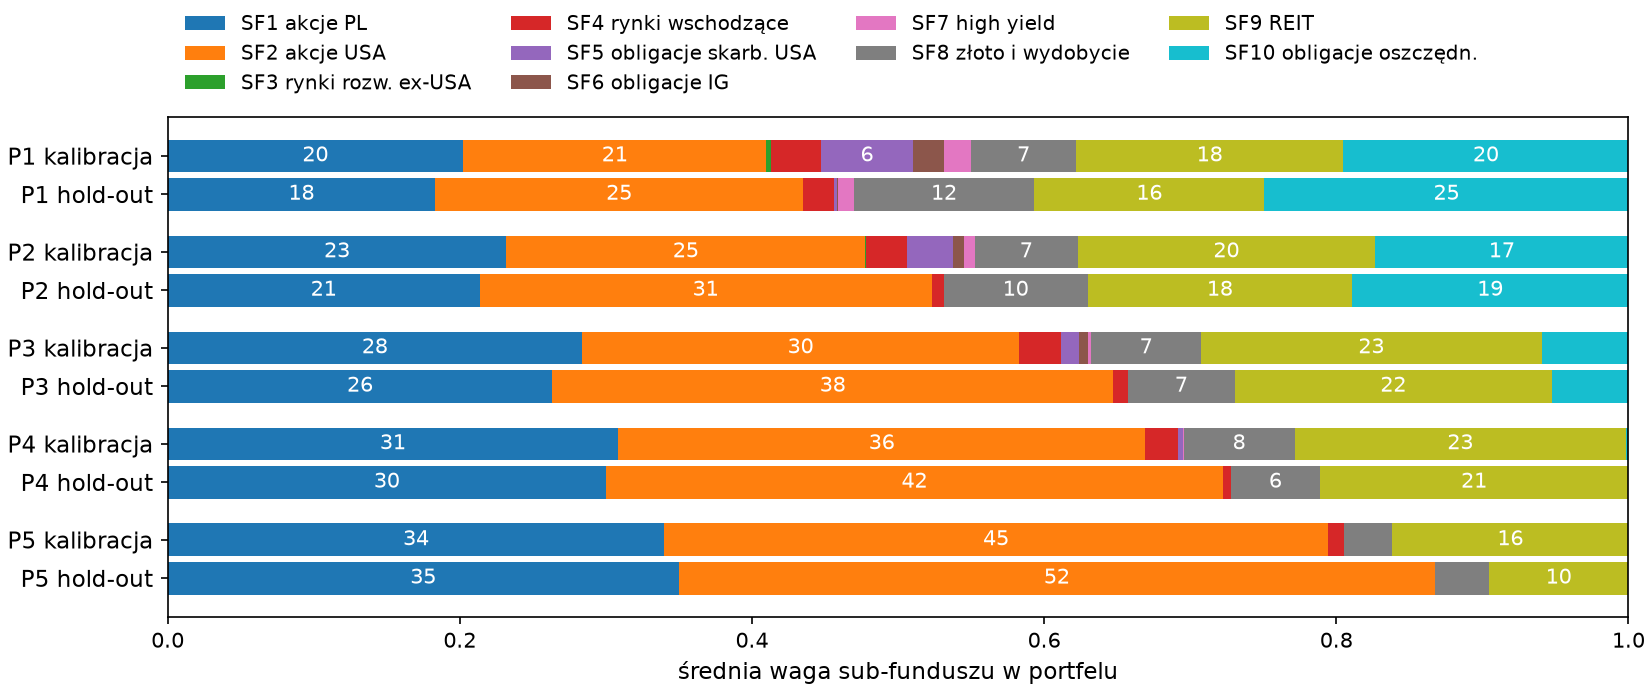
\includegraphics[width=.92\textwidth]{portfolio_W_mean.png}\par
  \raggedright\smallskip
  {\small Wraz ze spadkiem \(\gamma\) rośnie udział akcji (SF1+SF2:
    ok.\ 40\% w P1, ok.\ 87\% w P5 w hold-oucie), a znika SF10.}
  \srcmain{pipelines/composition_figures.py}{Kod wykresu: pipelines/composition\_figures.py}
\end{frame}

\begin{frame}{Ograniczenie look-through w praktyce}
  \centering
  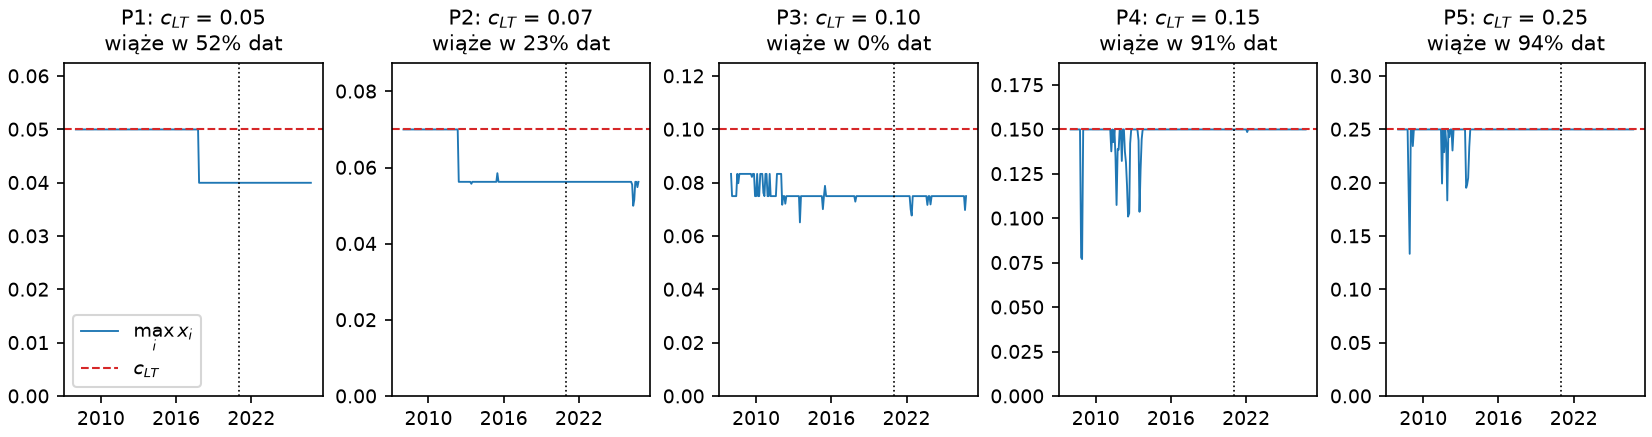
\includegraphics[width=\textwidth]{lookthrough_max_x.png}\par
  \raggedright\medskip
  \begin{itemize}
    \item P4--P5: \(\max_i x_i\) leży na limicie \(c_{LT}\) w 91--94\% dat;
      \(W_k\le c_{LT}/m_k\le0{,}50\), więc portfel trzyma 2--3 subfundusze.
    \item P1--P3: \(c_{SF}W_{\max}=0{,}04/0{,}056/0{,}075<c_{LT}\), więc
      wiąże \(W_{\max}\) (98--100\% dat), a \(c_{LT}\) tylko przy
      \(1/n_k>c_{SF}\) (0--52\% dat); mediana 6--8 subfunduszy.
  \end{itemize}
  \srcmain{pipelines/composition_figures.py}{Kod wykresu: pipelines/composition\_figures.py}
\end{frame}

% ============================================================ backtest i hold-out
\begin{frame}{Kroczący backtest i próba hold-out}
  \centering
  \begin{tikzpicture}[
    node distance=3.4mm,
    box/.style={draw=Teal,fill=Paper,rounded corners=2pt,
      text width=29mm,align=center,minimum height=13mm},
    >=Stealth]
    \node[box] (a) {Okno 1260 sesji do \(t-1\)};
    \node[box,right=of a] (b) {Modele, scenariusze, wagi, prognoza};
    \node[box,right=of b] (c) {Transakcja na zamknięciu \(t\)};
    \node[box,right=of c] (d) {Realizacja do \(t_{\text{next}}\), PIT straty};
    \draw[->,Teal] (a)--(b);
    \draw[->,Teal] (b)--(c);
    \draw[->,Teal] (c)--(d);
  \end{tikzpicture}
  \raggedright\medskip
  \begin{itemize}
    \item \textbf{Kalibracja} 2008--2020 (156 mies.), \textbf{hold-out}
      2021-01 -- 2026-09 (69 mies.).
    \item Przed pierwszą datą hold-outu zamrażamy parametry meta
      (\(\gamma,\kappa\), limity, \(q\), \(\varepsilon\), obcięcie vine'a)
      w \texttt{frozen\_params.json}; przebieg z inną konfiguracją
      jest odrzucany.
    \item W hold-oucie modele (GARCH, kopuły) są dalej estymowane co
      miesiąc w oknie kroczącym -- to część strategii, nie strojenie.
    \item Każda prognoza używa wyłącznie danych sprzed decyzji.
  \end{itemize}
  \src{pipelines/backtest.py}{Główny pipeline i konsolidacja wyników}
\end{frame}

\begin{frame}{Bootstrap w ocenie wyników hold-outu}
  \begin{columns}[T,onlytextwidth]
    \column{.55\textwidth}
    \textbf{MC ex post} na zrealizowanych dziennych stopach netto:
    \begin{itemize}
      \item \textbf{Bootstrap stacjonarny} \citep{politis1994}: bloki
        o długości \(\sim\mathrm{Geom}(1/b)\),
        \(b=\max\bigl(\hat b(r),\hat b(r^2)\bigr)\),
        \(\hat b\) wg \citet{politis2004}.
      \item \textbf{FHS} \citep{barone1999}: GJR-GARCH na szeregu, \(\varepsilon_h=\sigma_h\hat z^*\),
        \(\hat z^*\) losowane ze zwracaniem z reszt.
      \item Ścieżki 21-dniowe \(\Rightarrow\)
        \(R=\prod_h(1+r_h)-1\), ES ex post z SE.
    \end{itemize}
    {\small\textbf{Wnioskowanie:} MCS \citep{hansen2011}, 5000 repl.;
    różnica Sharpe'a \citep{ledoit2008}, blok 3 mies.\par}
    \column{.42\textwidth}
    \centering
    {\small ES 97,5\% [\%], R-vine \(\times\) \texttt{ce\_dep}, P3, hold-out}\par
    \smallskip
    \begin{tabular}{lr}
      \toprule
      Metoda & ES\\
      \midrule
      Prognoza ex ante (średnia) & 6,35\\
      Historyczne (69 mies.)     & 8,07\\
      MC wielowymiarowe          & 8,60\\
      Bootstrap stacjonarny      & 9,30\\
      FHS                        & 11,30\\
      \bottomrule
    \end{tabular}\par
    \smallskip
    \raggedright{\small Wszystkie metody ex post dają wyższe ES
      niż prognoza: model niedoszacowuje ogona.}
  \end{columns}
  \src{src/pf/backtest/expost_mc.py}{MC ex post: FHS i bootstrap stacjonarny}
\end{frame}

\begin{frame}{Przekroczenia VaR były częstsze, niż zakładał model}
  \centering
  {\small Średnia liczba przekroczeń miesięcznego VaR
    na poziomie 97,5\%}\par\medskip
  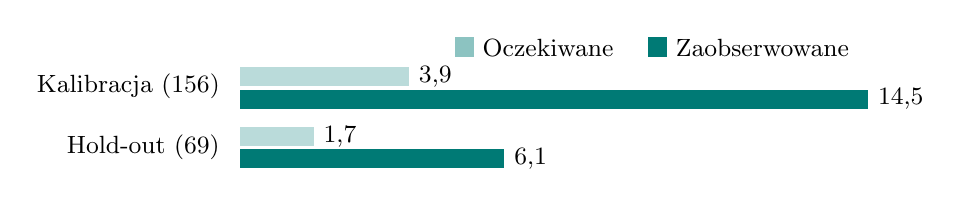
\begin{tikzpicture}[x=.55cm,y=.37cm,font=\small]
    \fill[Teal!27] (0,3.2) rectangle (3.9,3.85);
    \fill[Teal] (0,2.43) rectangle (14.5,3.08);
    \fill[Teal!27] (0,1.15) rectangle (1.7,1.8);
    \fill[Teal] (0,.38) rectangle (6.1,1.03);
    \node[anchor=east] at (-.25,3.18) {Kalibracja (156)};
    \node[anchor=east] at (-.25,1.1) {Hold-out (69)};
    \node[anchor=west] at (3.9,3.52) {3,9};
    \node[anchor=west] at (14.5,2.75) {14,5};
    \node[anchor=west] at (1.7,1.47) {1,7};
    \node[anchor=west] at (6.1,.7) {6,1};
    \node at (9.5,4.55)
      {\textcolor{Teal!45}{\rule{2.5mm}{2.5mm}} Oczekiwane
       \quad\textcolor{Teal}{\rule{2.5mm}{2.5mm}} Zaobserwowane};
  \end{tikzpicture}
  \raggedright\medskip
  \begin{itemize}
    \item Kupiec: \(\mathrm{LR}=-2\ln\frac{(1-p)^{T-n}p^{n}}
      {(1-\hat p)^{T-n}\hat p^{n}}\sim\chi^2_1\), \(p=1-\alpha\),
      \(\hat p=n/T\) \citep{kupiec1995}; \citet{christoffersen1998}
      -- niezależność przekroczeń.
    \item ES: test \(Z_2\) \citep{acerbi2014} i test na PIT
      \(u_t=\hat F_t(L_t)\) \citep{du2017}.
    \item Około 53\% przekroczeń w hold-oucie przypadło na 2022 r.;
      przy próbie miesięcznej moc testów jest niska.
  \end{itemize}
  \src{artifacts/reports/backtest_summary.md}{Raport przebiegu 7d0ff370e76f}
\end{frame}

\begin{frame}{Wpływ na alokację zależał od profilu}
  \centering
  {\small Zrealizowany CE w hold-oucie, \% rocznie, od zwrotów netto
    ponad WIBOR 1M:
    \(\mathrm{CE}=\bigl(\tfrac1T\sum_t(1+\tilde r_t)^{1-\gamma}\bigr)^{\frac1{1-\gamma}}-1\)}\par\medskip
  \begin{tabular}{lrrrrr}
    \toprule
    Profil & \texttt{ce\_dep} & \texttt{ce} & Równe wagi
           & Śr.--wariancja & SPY\\
    \midrule
    P1 & 2,53  & 2,31  & 3,08 & 2,57  & 2,49\\
    P2 & 3,96  & 4,24  & 4,09 & 4,25  & 5,20\\
    P3 & 5,44  & 5,94  & 4,77 & 5,61  & 7,03\\
    P4 & 5,88  & 6,92  & 5,45 & 8,43  & 8,88\\
    P5 & 13,02 & 13,12 & 5,96 & 11,42 & 10,28\\
    \bottomrule
  \end{tabular}
  \raggedright\smallskip
  \begin{itemize}
    \item Wyniki \texttt{ce\_dep} i \texttt{ce} uśredniono po
      siedmiu modelach. Obie strategie pobiły wszystkie benchmarki
      tylko w P5.
    \item Kara \(\kappa\) podnosi CE tylko w P1 (w kalibracji też w P2);
      MCS nie rozróżnia większości strategii.
  \end{itemize}
  \src{artifacts/reports/ranking_holdout.md}{Ranking hold-out przebiegu 7d0ff370e76f}
\end{frame}

% ============================================================ zakończenie
\begin{frame}{Cztery obszary pracy zespołu}
  \begin{enumerate}
    \item \textbf{Dane i statystyka opisowa.} Przygotowanie danych
      w PLN, kontrola jakości i dostępności historycznej.
    \item \textbf{Modelowanie.} Marginesy, kopuły i diagnostyka
      dopasowania.
    \item \textbf{Symulacje i ryzyko.} Scenariusze Monte Carlo,
      VaR i ES, optymalizacja oraz ocena prognoz poza próbą.
    \item \textbf{Aplikacja i wizualizacja.} Raportowanie wyników
      oraz plan integracji z interfejsem Streamlit i ankietą.
  \end{enumerate}
  \src{README.md}{Struktura repozytorium i format wyników}
\end{frame}

\begin{frame}{Wnioski}
  \begin{enumerate}
    \item \textbf{Modelowanie.} R-vine ma najlepsze BIC i jako jedyny
      należy do MCS według log-score poza próbą, ale najlepsze portfele
      w hold-oucie dały C-vine (P1, P2, P4) i kopuła Gaussa (P5).
    \item \textbf{Użyteczność.} Kara za zależność w ogonie zwiększa CE
      tylko przy najwyższym \(\gamma\) (P1), w pozostałych profilach obniża.
    \item \textbf{Struktura.} Koncentrację w P4--P5 wyznacza limit
      look-through \(c_{LT}\) (głównie SF1 i SF2), w P1--P3 limit
      \(W_{\max}\).
    \item \textbf{Ryzyko.} Prognozy ES są zaniżone względem bootstrapu
      i FHS ex post, a przekroczeń VaR jest ok.\ 3,5--4 razy więcej
      niż oczekiwano.
  \end{enumerate}
  \begin{block}{Trzy kryteria oceny}
    Dopasowanie kopuły, trafność prognozy ryzyka i wynik portfela
    mierzą różne aspekty działania modelu.
  \end{block}
  \src{README.md}{Wyniki, interpretacja i ograniczenia badania}
\end{frame}

% ============================================================ bibliografia
\begin{frame}[allowframebreaks]{Bibliografia}
  \scriptsize
  \begin{thebibliography}{99}
    \setlength{\itemsep}{1pt}
    \bibitem[Aas i in.(2009)]{aas2009}
      Aas, K., Czado, C., Frigessi, A., Bakken, H. (2009).
      Pair-copula constructions of multiple dependence.
      \emph{Insurance: Mathematics and Economics}, 44(2), 182--198.
    \bibitem[Acerbi i Székely(2014)]{acerbi2014}
      Acerbi, C., Székely, B. (2014). Backtesting expected shortfall.
      \emph{Risk}, 27(11), 76--81.
    \bibitem[Acerbi i Tasche(2002)]{acerbi2002}
      Acerbi, C., Tasche, D. (2002). On the coherence of expected shortfall.
      \emph{Journal of Banking \& Finance}, 26(7), 1487--1503.
    \bibitem[Artzner i in.(1999)]{artzner1999}
      Artzner, P., Delbaen, F., Eber, J.-M., Heath, D. (1999).
      Coherent measures of risk. \emph{Mathematical Finance}, 9(3), 203--228.
    \bibitem[Barone-Adesi i in.(1999)]{barone1999}
      Barone-Adesi, G., Giannopoulos, K., Vosper, L. (1999).
      VaR without correlations for portfolios of derivative securities.
      \emph{Journal of Futures Markets}, 19(5), 583--602.
    \bibitem[Bedford i Cooke(2002)]{bedford2002}
      Bedford, T., Cooke, R.\,M. (2002). Vines -- a new graphical model for
      dependent random variables. \emph{Annals of Statistics}, 30(4), 1031--1068.
    \bibitem[Bo\c{t}oc(2017)]{botoc2017}
      Bo\c{t}oc, C. (2017). Univariate and bivariate volatility in Central
      European stock markets. \emph{Prague Economic Papers}, 26(2), 127--141.
    \bibitem[Christoffersen(1998)]{christoffersen1998}
      Christoffersen, P.\,F. (1998). Evaluating interval forecasts.
      \emph{International Economic Review}, 39(4), 841--862.
    \bibitem[Dißmann i in.(2013)]{dissmann2013}
      Dißmann, J., Brechmann, E.\,C., Czado, C., Kurowicka, D. (2013).
      Selecting and estimating regular vine copulae and application to
      financial returns. \emph{Computational Statistics \& Data Analysis},
      59, 52--69.
    \bibitem[Du i Escanciano(2017)]{du2017}
      Du, Z., Escanciano, J.\,C. (2017). Backtesting expected shortfall:
      accounting for tail risk. \emph{Management Science}, 63(4), 940--958.
    \bibitem[Embrechts i in.(2002)]{embrechts2002}
      Embrechts, P., McNeil, A.\,J., Straumann, D. (2002). Correlation and
      dependence in risk management: properties and pitfalls. W:
      M.\,A.\,H. Dempster (red.), \emph{Risk Management: Value at Risk and
      Beyond}, Cambridge University Press, 176--223.
    \bibitem[Glosten i in.(1993)]{glosten1993}
      Glosten, L.\,R., Jagannathan, R., Runkle, D.\,E. (1993). On the relation
      between the expected value and the volatility of the nominal excess
      return on stocks. \emph{Journal of Finance}, 48(5), 1779--1801.
    \bibitem[Hansen(1994)]{hansen1994}
      Hansen, B.\,E. (1994). Autoregressive conditional density estimation.
      \emph{International Economic Review}, 35(3), 705--730.
    \bibitem[Hansen i in.(2011)]{hansen2011}
      Hansen, P.\,R., Lunde, A., Nason, J.\,M. (2011). The model confidence
      set. \emph{Econometrica}, 79(2), 453--497.
    \bibitem[Kupiec(1995)]{kupiec1995}
      Kupiec, P.\,H. (1995). Techniques for verifying the accuracy of risk
      measurement models. \emph{Journal of Derivatives}, 3(2), 73--84.
    \bibitem[Kurach i Papla(2016)]{kurach2016}
      Kurach, R., Papla, D. (2016). Should pension funds hedge currency risk?
      The case of Poland. \emph{Baltic Journal of Economics}, 16(2), 81--94.
    \bibitem[Ledoit i Wolf(2004)]{ledoit2004}
      Ledoit, O., Wolf, M. (2004). A well-conditioned estimator for
      large-dimensional covariance matrices. \emph{Journal of Multivariate
      Analysis}, 88(2), 365--411.
    \bibitem[Ledoit i Wolf(2008)]{ledoit2008}
      Ledoit, O., Wolf, M. (2008). Robust performance hypothesis testing with
      the Sharpe ratio. \emph{Journal of Empirical Finance}, 15(5), 850--859.
    \bibitem[McNeil i Frey(2000)]{mcneil2000}
      McNeil, A.\,J., Frey, R. (2000). Estimation of tail-related risk
      measures for heteroscedastic financial time series: an extreme value
      approach. \emph{Journal of Empirical Finance}, 7(3--4), 271--300.
    \bibitem[McNeil i in.(2005)]{mcneil2005}
      McNeil, A.\,J., Frey, R., Embrechts, P. (2005). \emph{Quantitative Risk
      Management: Concepts, Techniques and Tools}. Princeton University Press.
    \bibitem[Müller i Righi(2024)]{muller2024}
      Müller, F.\,M., Righi, M.\,B. (2024). Comparison of Value at Risk (VaR)
      multivariate forecast models. \emph{Computational Economics}, 63,
      75--110.
    \bibitem[Politis i Romano(1994)]{politis1994}
      Politis, D.\,N., Romano, J.\,P. (1994). The stationary bootstrap.
      \emph{Journal of the American Statistical Association}, 89(428),
      1303--1313.
    \bibitem[Politis i White(2004)]{politis2004}
      Politis, D.\,N., White, H. (2004). Automatic block-length selection for
      the dependent bootstrap. \emph{Econometric Reviews}, 23(1), 53--70.
    \bibitem[Pratt(1964)]{pratt1964}
      Pratt, J.\,W. (1964). Risk aversion in the small and in the large.
      \emph{Econometrica}, 32(1--2), 122--136.
    \bibitem[Rockafellar i Uryasev(2000)]{rockafellar2000}
      Rockafellar, R.\,T., Uryasev, S. (2000). Optimization of conditional
      value-at-risk. \emph{Journal of Risk}, 2(3), 21--41.
    \bibitem[Sheppard i in.(2024)]{arch}
      Sheppard, K. i in. (2024). \emph{arch: ARCH models, bootstrap and
      multiple comparison procedures in Python} (oprogramowanie, wersja 7).
      Zenodo, doi:10.5281/zenodo.593254.
    \bibitem[Sklar(1959)]{sklar1959}
      Sklar, A. (1959). Fonctions de répartition à \(n\) dimensions et leurs
      marges. \emph{Publications de l'Institut de Statistique de
      l'Université de Paris}, 8, 229--231.
    \bibitem[Virtanen i in.(2020)]{scipy2020}
      Virtanen, P. i in. (2020). SciPy 1.0: fundamental algorithms for
      scientific computing in Python. \emph{Nature Methods}, 17, 261--272.
    \bibitem[Vuong(1989)]{vuong1989}
      Vuong, Q.\,H. (1989). Likelihood ratio tests for model selection and
      non-nested hypotheses. \emph{Econometrica}, 57(2), 307--333.
  \end{thebibliography}
\end{frame}

\begin{frame}{Źródła w repozytorium}
  \begin{itemize}
    \item \href{\repo/tree/\rev}{Kod i README, rewizja \texttt{9e941db}}
    \item \href{\repo/blob/\rev/docs/backtest.md}{Metodologia backtestu}
    \item \href{\repo/blob/\rev/docs/dependence_model.md}{Modele zależności}
    \item \href{\repo/blob/\rev/artifacts/reports/backtest_summary.md}
      {Podsumowanie backtestu}
    \item \href{\repo/blob/\rev/artifacts/reports/es_mc.md}
      {MC ex post: VaR i ES}
    \item \href{\repo/blob/main/pipelines/composition_figures.py}
      {Kod wykresów struktury funduszu}
  \end{itemize}
  \vfill
  {\color{Teal}\Large Dziękujemy za uwagę}
\end{frame}

\end{document}
